\section{Una de ordenar código}

El cine Peliculandia guarda en un archivo de texto \texttt{entradas.txt} los datos personales de los espectadores que compran entradas para las funciones y la información de la película que vieron. Cada línea tiene el formato de \texttt{nombre;edad;pelicula;duracion}. 

\begin{figure}[h]
    \centering
    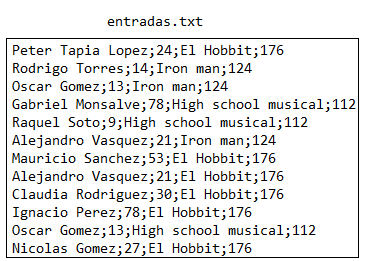
\includegraphics[scale=0.9]{Guia/entradas.png}
\end{figure}

Este cine discrimina los precios de las entradas de las distintas personas, a los menores de 15 años cobra 1500, a los mayores de 65 años cobra 2000 y a público general (entre 15 y 65 años) cobra 3500.
\\
Se quiere saber, mediante dos funciones, cuanto es el ingreso total reflejado en el archivo \texttt{entradas.txt} y quien es el espectador que más tiempo ha estado en el cine (en base a la duración de las películas que ha visto). Se le pide a usted ordenar e indentar (dejar los espacios correspondientes en python) las líneas de código que forman las funciones.

\begin{figure}[h]
    \centering
    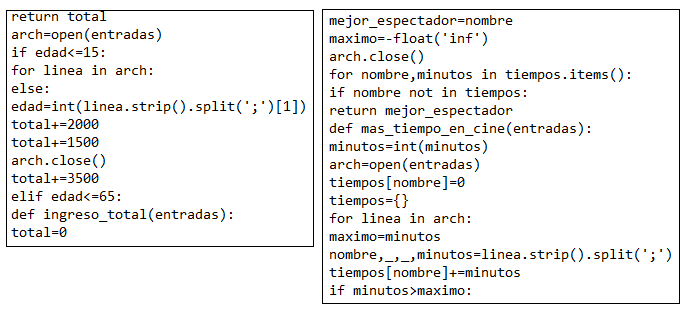
\includegraphics[scale=0.9]{Guia/funciones.png}
\end{figure}